\begin{frame}{L1 — the measurement information model}
	\begin{columns}[T]
		\begin{column}{0.62\textwidth}
			\centering
			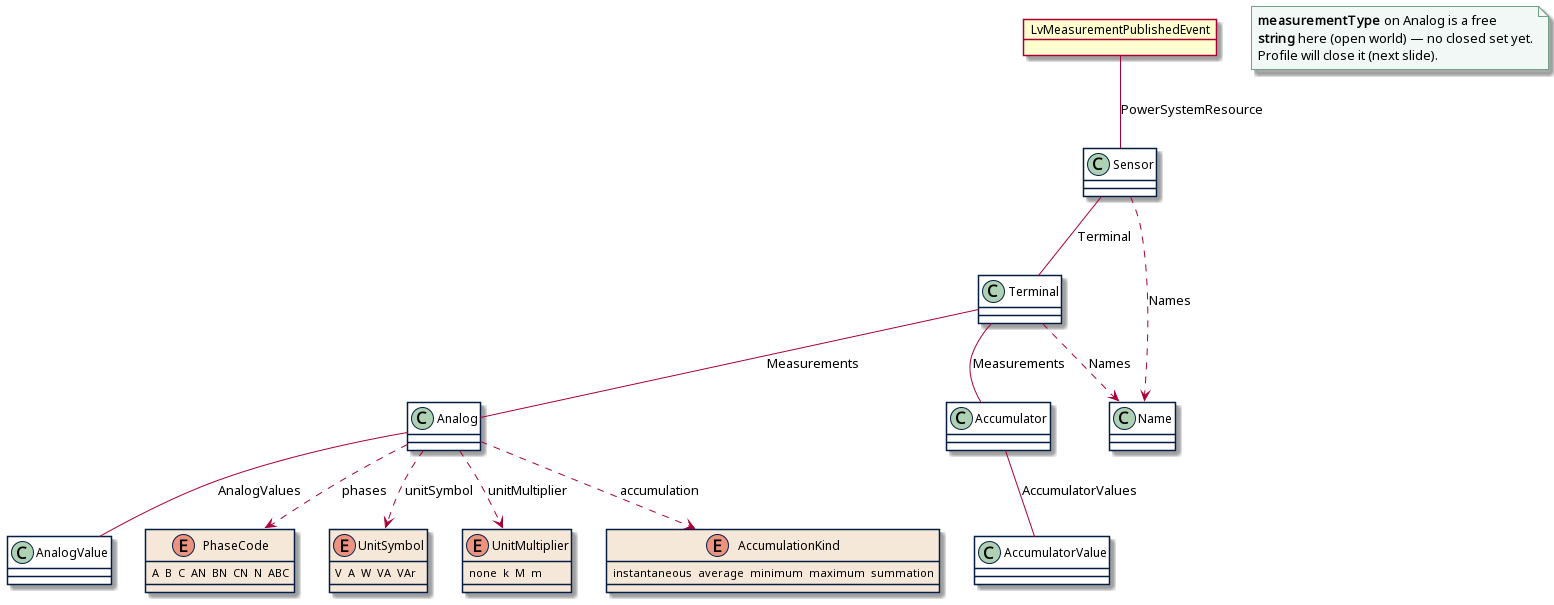
\includegraphics[width=\linewidth]{slides/exchange/example-information-model/figs/information-model.png}
		\end{column}
		\begin{column}{0.38\textwidth}
			\textbf{Everything here is standard or convention:}
			\begin{itemize}
				\scriptsize
				\item \texttt{Sensor, Terminal, Analog, Accumulator, AnalogValue} — CIM core classes (IEC 61970-301)
				\item \texttt{PhaseCode, UnitSymbol, UnitMultiplier} — CIM enumerations
				\item \texttt{mRID} — IEC 61970-552 identifier convention
				\item \texttt{QualityMetadata} — W3C DQV, re-used
			\end{itemize}
		\end{column}
	\end{columns}
	\vspace{0.3em}
	\alert{Nothing local, nothing proprietary.} This is what we get for free —
	the definitions our engineers currently re-type into every schema file.
\end{frame}
